\documentclass[aspectratio=169,xcolor=dvipsnames]{beamer}
\usetheme{SimpleDarkBlue}

\usepackage{hyperref}
\usepackage{graphicx}
\usepackage{booktabs}
\usepackage{amssymb}
\usepackage{amsmath}
\usepackage{tikz}
\usepackage{xcolor}
\usepackage{caption}
\usepackage{amsthm}

\title{Graph RAG}
\author{Mohammad Hosein Rabiee \and Amir Hosein Karimzadgan}
\institute{Department of Computer Science and Statistics \\ Faculty of Mathematics \\ K. N. Toosi University of Technology}
\date{}

\begin{document}
	
	\begin{frame}
		\titlepage
	\end{frame}
	
	\begin{frame}{Overview}
		
		\vspace{0.6em}
		
		\begin{enumerate}
			\item \textbf{Introduction to Graph RAG:} motivation, main use cases, and core methods
			\item \textbf{Use Case I:} Enhancing multi‑hop question answering performance
			\item \textbf{Use Case II:} Global summarization of large document collections
			\item \textbf{The Gap:} Current GraphRAG requires exposing raw sensitive data to external LLMs
		\end{enumerate}
		
	\end{frame}
	
	\begin{frame}{Defining Retrieval-Augmented Generation (RAG)}
		
		\small
		
		\begin{itemize}
			\item \textbf{\textcolor{blue!80}{What is RAG?}}  
			RAG is a technique that supplements Large Language Models (LLMs) with external knowledge to enhance factual accuracy and trustworthiness.
			
			\vspace{0.2cm}
			
			\item \textbf{\textcolor{blue!80}{The Core Process:}}  
			It typically involves two major steps:
			\begin{itemize}
				\item \textbf{\textcolor{teal!80}{Retrieval:}}  
				Given a user question, the system uses an index to find the most relevant chunks of information from a large corpus.
				
				\item \textbf{\textcolor{teal!80}{Generation:}}  
				The LLM uses these retrieved chunks as context to generate an informed response.
			\end{itemize}
			
			\vspace{0.2cm}
			
			\item \textbf{\textcolor{blue!80}{The Problem it Solves:}}  
			RAG mitigates \textbf{\textcolor{red!70}{hallucinations}}, which occur when LLMs generate incorrect outputs due to missing domain-specific, real-time, or proprietary knowledge.
		\end{itemize}
		
	\end{frame}
	
	\begin{frame}{Why We Use Graph-Based RAG}
		
		\small
		
		\begin{itemize}
			\item \textbf{\textcolor{blue!80}{Limitation of Vanilla RAG:}}  
			Standard RAG retrieves knowledge directly from isolated text chunks, which may fail to capture rich semantic links between entities.
			
			\vspace{0.2cm}
			
			\item \textbf{\textcolor{blue!80}{The Graph Advantage:}}  
			Graph-based RAG employs graph structures (nodes and edges) built from the corpus to enhance contextual understanding.
			
			\vspace{0.2cm}
			
			\item \textbf{\textcolor{blue!80}{Key Benefits:}}
			\begin{itemize}
				\item \textbf{\textcolor{teal!80}{Captures Relationships:}}  
				Explicitly models links between entities (e.g., Real Sociedad winning Copa Del Rey in a specific year).
				
				\item \textbf{\textcolor{teal!80}{Improved Accuracy:}}  
				Enhances factual accuracy, adaptability, and interpretability.
				
				\item \textbf{\textcolor{teal!80}{Structured Representation:}}  
				Edges can be enriched with contextual properties such as temporal data and attributes.
			\end{itemize}
		\end{itemize}
		
	\end{frame}
	
	\begin{frame}{Vanilla RAG vs. Graph-based RAG}
		
		\begin{figure}
			\centering
			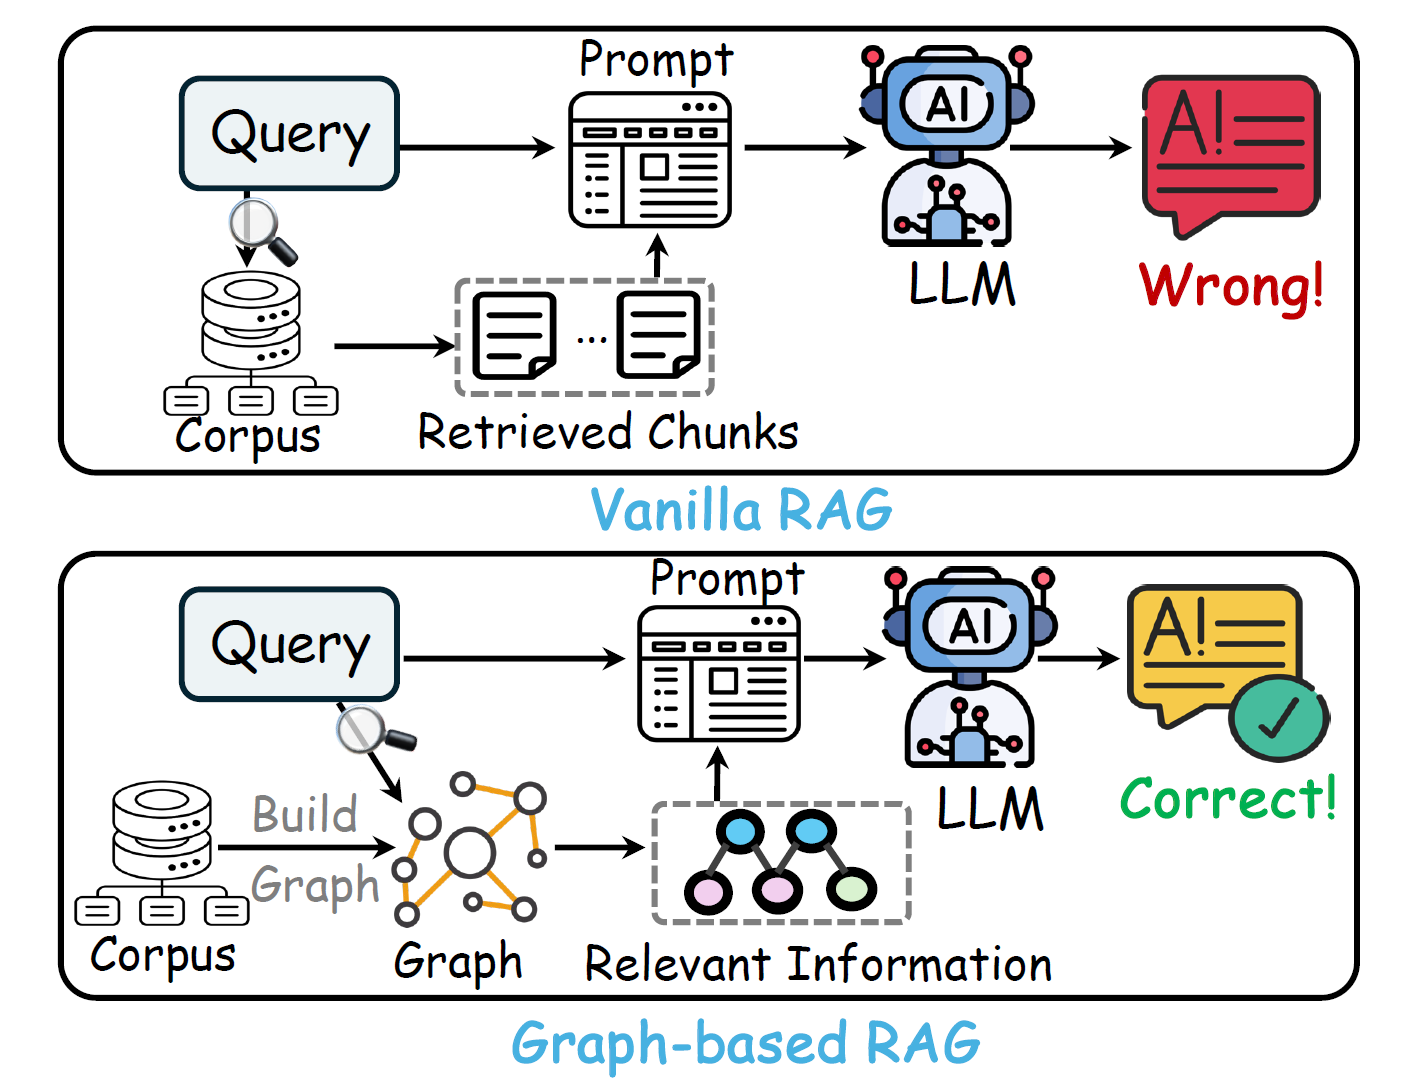
\includegraphics[width=0.6\linewidth]{images/figure1.png}
			\caption{Overview of vanilla RAG and graph-based RAG.}
		\end{figure}
		
		\vspace{0.5em}
		
	\end{frame}
	
	\begin{frame}{Introducing the Unified Framework}
		
		\small
		
		\begin{itemize}
			\item \textbf{\textcolor{blue!80}{Overview:}}  
			To systematically compare different methods, the sources propose a unified framework consisting of four distinct stages  
			\alert{\cite{zhou2025graphRAG}}:
			
			\vspace{0.2cm}
			
			\begin{enumerate}
				\item \textbf{\textcolor{teal!80}{Graph Building:}}  
				Transforming the input corpus into a graph (e.g., Knowledge Graph, Tree, or Passage Graph) by extracting nodes and edges.
				
				\item \textbf{\textcolor{teal!80}{Index Construction:}}  
				Storing graph elements (nodes, relationships, or communities) in a vector database or computing community reports.
				
				\item \textbf{\textcolor{teal!80}{Operator Configuration:}}  
				Selecting retrieval operators (e.g., Vector Search, Personalized PageRank).
				
				\item \textbf{\textcolor{teal!80}{Retrieval \& Generation:}}  
				Converting the user question into a searchable unit and generating the final answer.
			\end{enumerate}
		\end{itemize}
		
	\end{frame}
	
	\begin{frame}{Unified Framework of Graph-based RAG}
		
		\begin{figure}
			\centering
			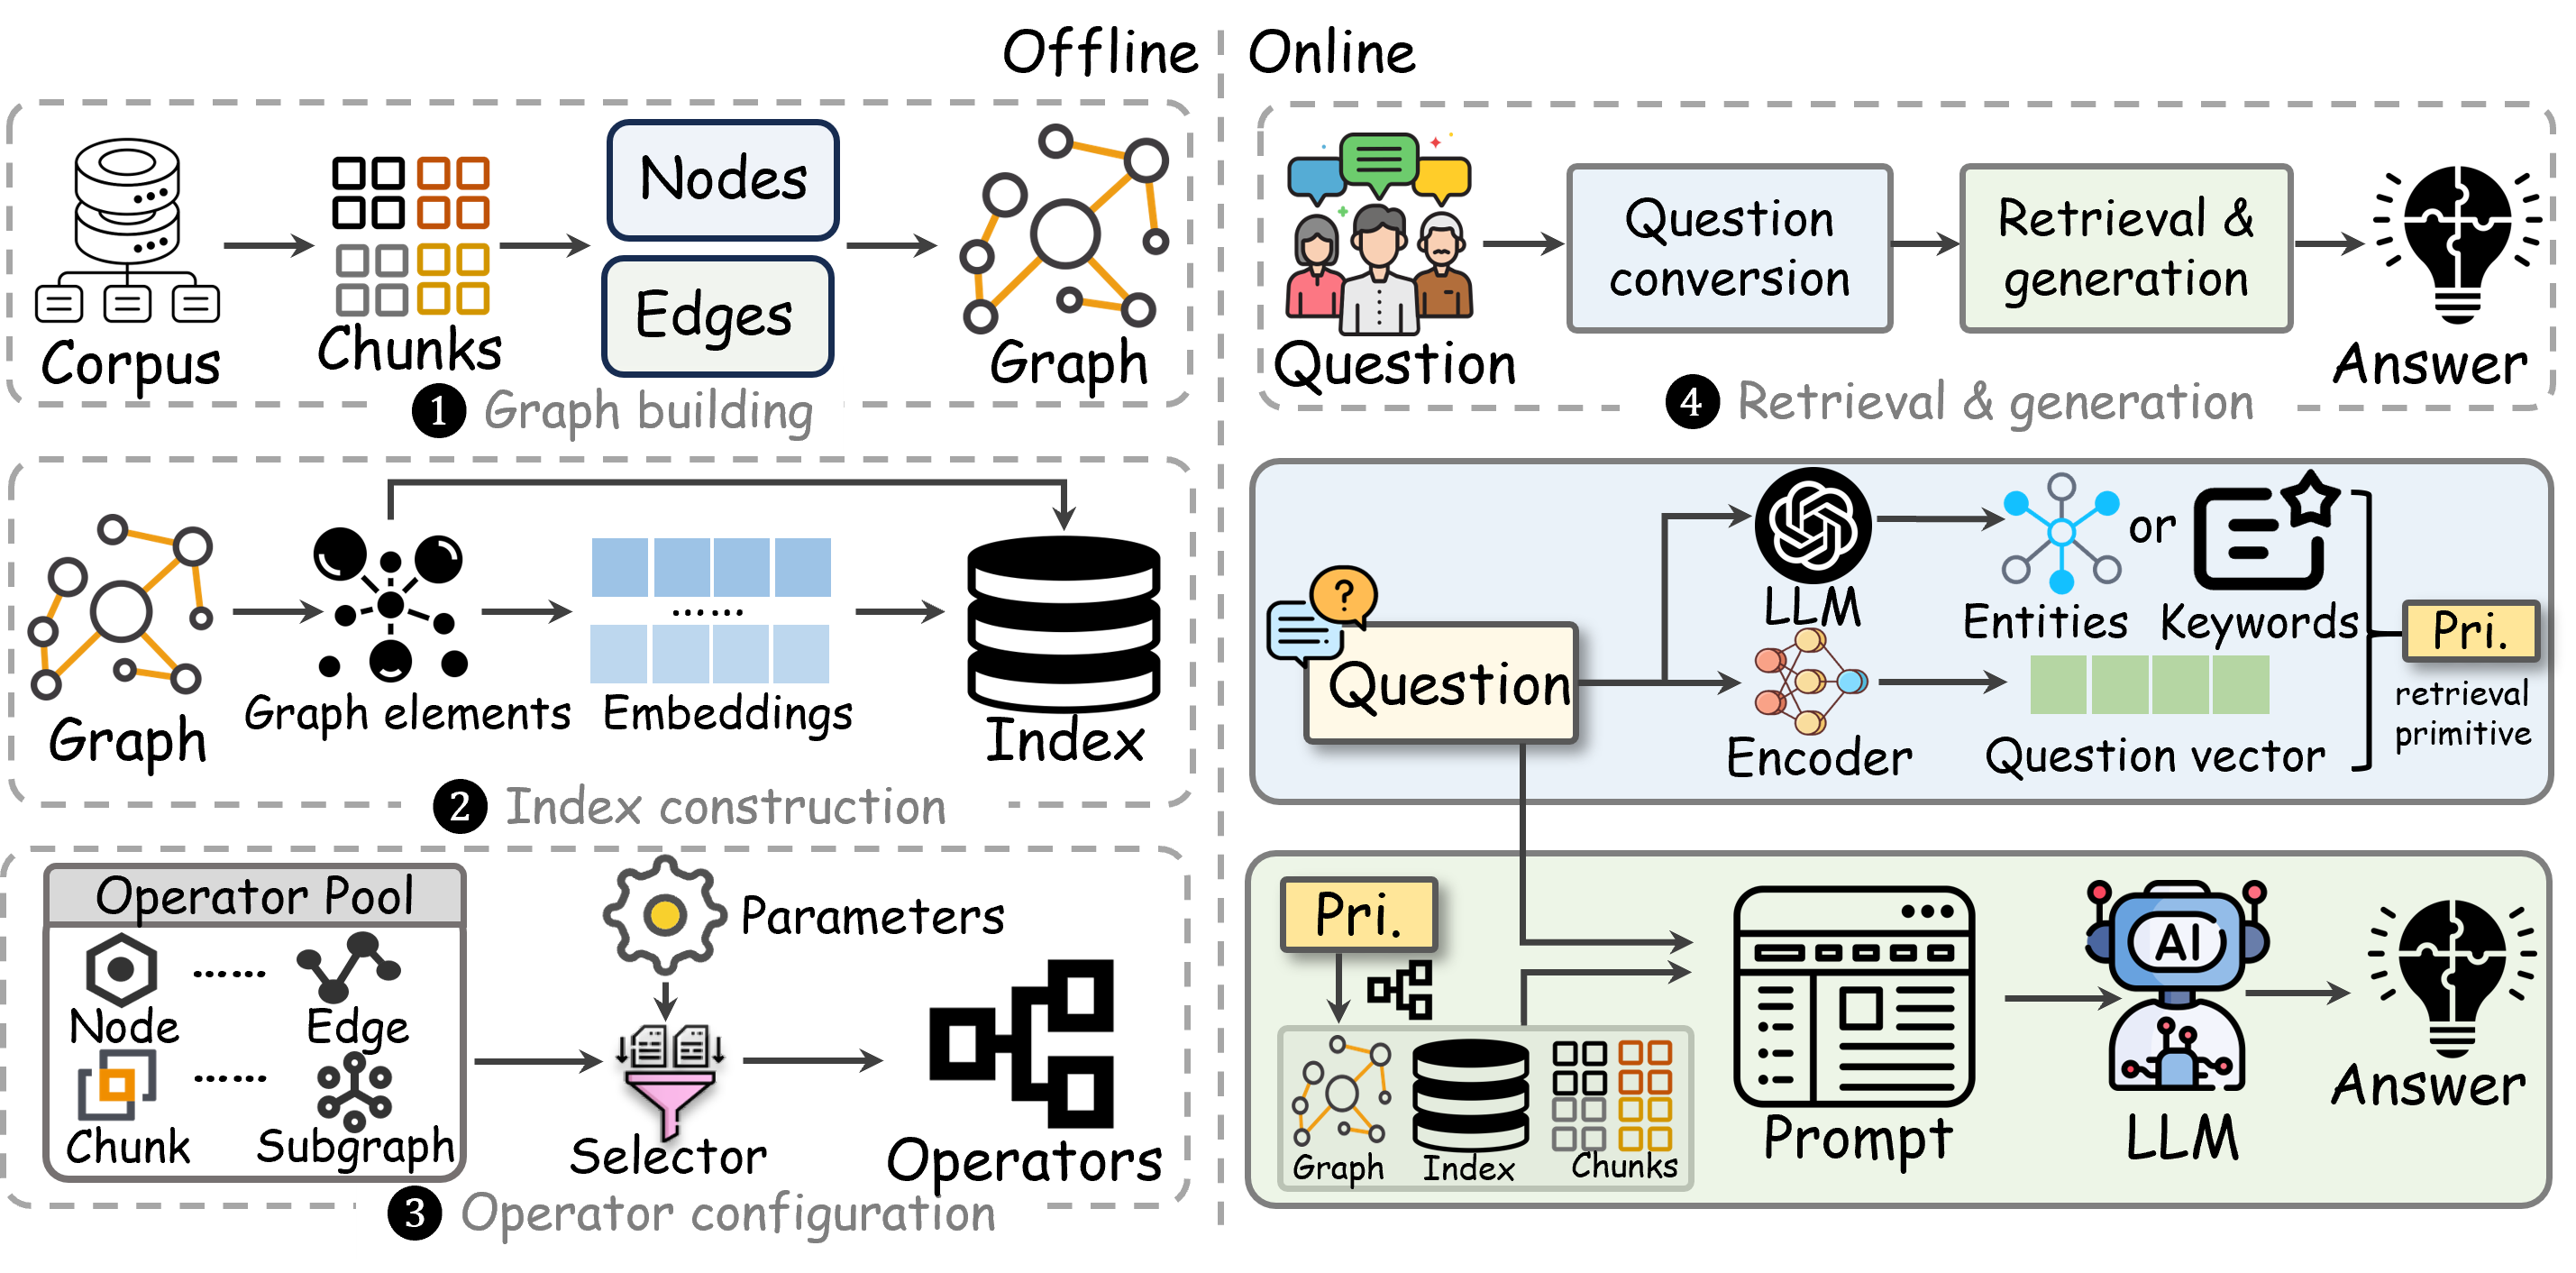
\includegraphics[width=0.95\linewidth]{images/figure2.png}
			\caption{Workflow of graph-based RAG methods under a unified framework.}
		\end{figure}
		
	\end{frame}
	
	\begin{frame}{Challenges in Multi-Hop Question Answering}
		
		\begin{block}{Definition}
			Multi-hop QA requires reasoning over multiple pieces of information
			or documents to answer complex queries.
		\end{block}
		
		\begin{itemize}
			\item \textbf{Core Difficulties:}
			\begin{itemize}
				\item Necessitates multi-step reasoning.
				\item Requires integration of information from disparate sources.
			\end{itemize}
			
			\item \textbf{Shortcomings of Existing Methods:}
			Traditional approaches often struggle with effective retrieval across documents,
			leading to incomplete or inaccurate answers.
			
			\item \textbf{The MuSiQue Dataset:}
			A benchmark designed for 2--4 hop questions to improve performance
			on genuine multihop tasks.
		\end{itemize}
		
	\end{frame}
	
	\begin{frame}{Research Gap and Proposed Solution}
		
		\begin{itemize}
			\item \textbf{The Problem:}
			Traditional RAG models often fail to integrate information from
			disparate sources into coherent and accurate answers for multi-hop tasks.
			
			\item \textbf{Proposed Innovation:}
			A novel approach leveraging vector embedding retrieval from a
			graph relations database. 	\alert{\cite{amiriShavaki2024kgRAGAVIR}}
			
			\item \textbf{Mechanism:}
			By constructing a knowledge graph and embedding its relations,
			the method explicitly models relationships between entities and
			concepts to enhance multi-hop reasoning.
		\end{itemize}
	\end{frame}
	
	\begin{frame}{Overall Pipeline}
		\centering
		
		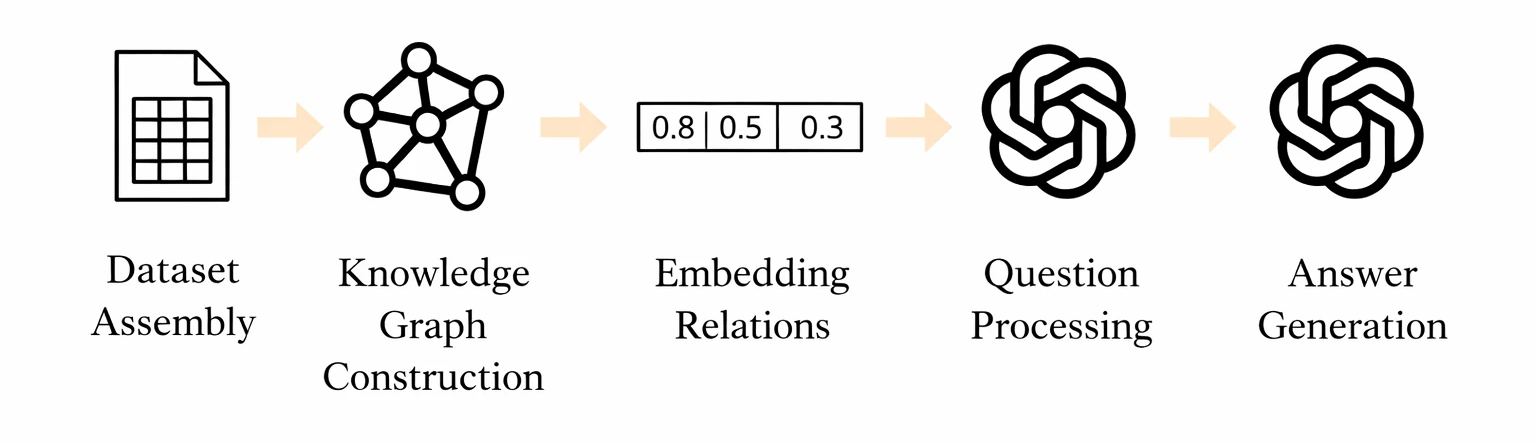
\includegraphics[width=\textwidth]{images/overall_pipeline.png}
		
	\end{frame}
	
	\begin{frame}{Dataset Assembly and Composition}
		
		\begin{columns}[T]
			
			\begin{column}{0.55\textwidth}
				
				\begin{itemize}
					\item \textbf{Scale:}
					The dataset consists of
					\textcolor{blue}{500 short textual documents} and
					\textcolor{blue}{296 multi-hop questions}.
					
					\item \textbf{Multi-Hop Requirement:}
					Questions are specifically designed so that
					\textcolor{red}{no single document contains the full answer};
					retrieval of \textcolor{red}{at least two documents} is required.
					
					\item \textbf{Data Sources:}
					\begin{itemize}
						\item \textcolor{teal}{20\% (100 documents):}
						Sourced from real-world internet texts.
						\item \textcolor{orange}{80\% (400 documents):}
						Generated by an LLM and validated by human supervisors.
					\end{itemize}
					
				\end{itemize}
				
			\end{column}
			
			\begin{column}{0.45\textwidth}
				
				\begin{itemize}
					\item \textbf{Purpose:}
					This curated dataset serves as a
					\textcolor{purple}{benchmark} to compare the proposed
					\textcolor{purple}{Graph RAG} method against
					\textcolor{purple}{traditional RAG approaches}.
				\end{itemize}
				\vspace{0.2cm}
				\centering
				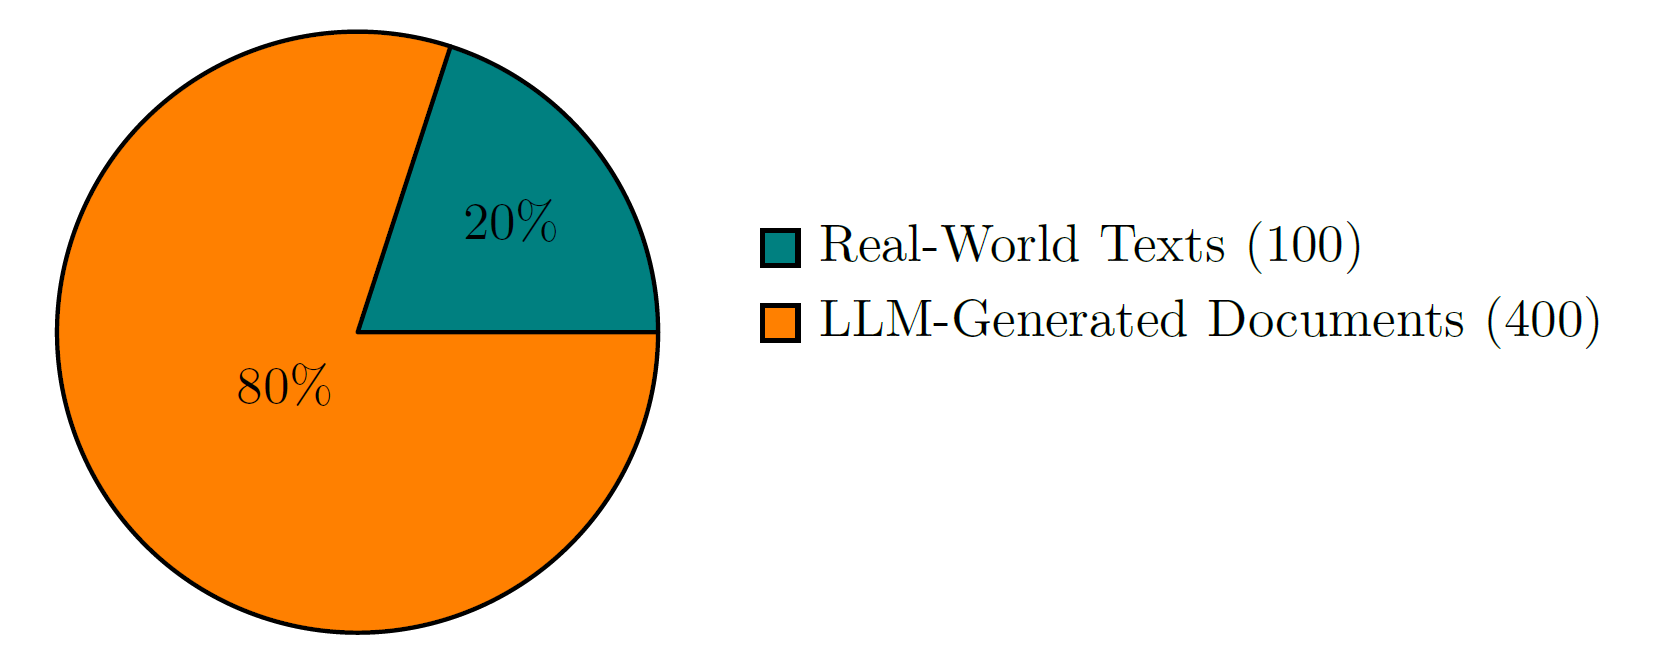
\includegraphics[width=\textwidth]{images/dataset.png}
				
				\vspace{0.2cm}
				{\footnotesize \textit{Composition of the dataset.}}
			\end{column}
			
		\end{columns}
		
	\end{frame}
	
	\begin{frame}{Knowledge Graph Construction}
		
		\small
		\begin{itemize}
			
			\item \textbf{\textcolor{blue}{Extraction Process}:}
			An LLM extracts entities
			(\textcolor{teal}{represented as nodes})
			and relationships
			(\textcolor{orange}{represented as edges})
			from the documents.
			
			\vspace{0.15cm}
			
			\item \textbf{\textcolor{purple}{Merging Methodology}:}
			\begin{itemize}
				\item Documents are processed
				\textcolor{purple}{individually}
				to extract relations.
				\item Individual graphs are then
				\textcolor{purple}{merged}
				into a unified, comprehensive graph.
			\end{itemize}
			
			\vspace{0.15cm}
			
			\item \textbf{\textcolor{red}{Efficiency Finding}:}
			Research indicated that merging separate graphs captures relations
			\textcolor{red}{more accurately} than attempting a single
			large-batch LLM extraction, which risks missing
			\textcolor{red}{critical connections}.
			
			\vspace{0.15cm}
			\item \textbf{\textcolor{blue}{Contextual Properties}:}
			Beyond simple nodes and edges, the graph stores
			\textcolor{blue}{temporal data (dates/times)} and
			\textcolor{blue}{attributes} as properties.
			
			\vspace{0.15cm}
			
			\item \textbf{\textcolor{teal}{Management}:}
			\textcolor{teal}{Neo4j} is used as the graph database to manage
			these complex, interconnected data structures.
			
		\end{itemize}
		
	\end{frame}
	
	\begin{frame}{Enriched Semantic Representation}
		
		\begin{columns}[T,onlytextwidth]
			
			\begin{column}{0.55\textwidth}
				\small
				
				\vspace{0.2cm}
				
				\begin{alertblock}{\textbf{Example}}
					\begin{itemize}
						\item \textbf{Relation 1:}
						(\textcolor{teal}{Real Sociedad},
						\textcolor{orange}{WON},
						\textcolor{teal}{Copa Del Rey}) with property
						\textcolor{red}{year = 2020}.
						\item \textbf{Relation 2:}
						(\textcolor{teal}{Real Sociedad},
						\textcolor{orange}{SHIRT\_COLOUR},
						\textcolor{teal}{Blue And White}).
					\end{itemize}
				\end{alertblock}
				
				\vspace{0.2cm}
				
				\begin{itemize}
					\item \textbf{\textcolor{purple}{Reasoning Capability}:}
					This structure allows the system to answer complex queries like
					\textcolor{red}{\textit{“What color did the 2020 Copa del Rey winners wear?”}}
					by navigating through specific properties.
				\end{itemize}
				
			\end{column}
			
			\begin{column}{0.45\textwidth}
				\centering
				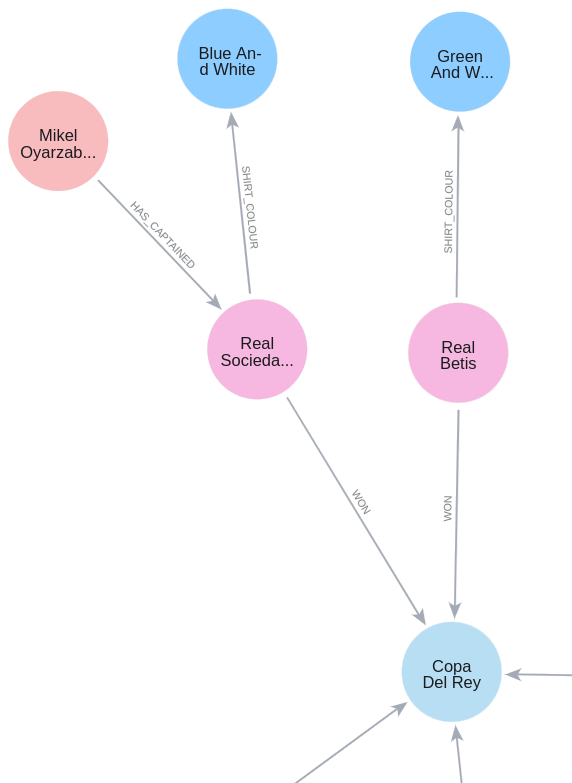
\includegraphics[width=0.7\textwidth]{images/subgraph.png}
				
				\vspace{0.2cm}
				{\footnotesize
					\textit{Sample subgraph of the constructed knowledge graph.}}
			\end{column}
			
		\end{columns}
		
	\end{frame}
	
	\begin{frame}{Embedding Relations in a Vector Database}
		
		\small
		\begin{itemize}
			
			\item \textbf{\textcolor{blue}{RAG-based Retrieval}}
			
			For the retrieval step, relations in the
			\textcolor{teal}{knowledge graph} are embedded into a
			\textcolor{blue}{vector database} to enable
			fast \textcolor{blue}{similarity search}.
			
			\vspace{0.15cm}
			
			\item \textbf{\textcolor{purple}{Structured Embedding Construction}}
			
			To create the embeddings, we use:
			\begin{itemize}
				\item the names of the two \textcolor{teal}{head entities},
				\item the \textcolor{orange}{relation} itself,
				\item and all associated \textcolor{purple}{properties}
				(including dates and times).
			\end{itemize}
			
			\vspace{0.15cm}
			
			\item \textbf{\textcolor{teal}{Context Retention}}
			
			Including \textcolor{teal}{temporal information} ensures that
			important context is preserved during retrieval.
			
			\vspace{0.15cm}
			
			\item \textbf{\textcolor{red}{Vector Storage and Similarity Search}}
			
			\begin{itemize}
				\item \textcolor{red}{FAISS} is used for efficient indexing based on
				approximate search algorithms.
				\item Retrieval is performed using
				\textcolor{red}{Euclidean distance (L2 norm)} to identify
				semantically similar relations.
			\end{itemize}
			
		\end{itemize}
		
	\end{frame}
	
	\begin{frame}{Answer Generation Workflow}
		
		\begin{columns}
			
			\column{0.65\textwidth}
			\small
			\begin{itemize}
				
				\item \textbf{\textcolor{blue}{Step 1: Identifying Incomplete Relations}}
				
				The user query is passed to an LLM, which identifies
				\textcolor{blue}{missing or incomplete relations}
				required to answer the question.
				
				\item \textbf{\textcolor{purple}{Step 2: Grounded Retrieval}}
				
				The vector database retrieves the most
				\textcolor{purple}{relevant relation embeddings}
				to complete the missing connections using
				\textcolor{purple}{similarity search}.
				
				\item \textbf{\textcolor{teal}{Step 3: Grounded Answer Synthesis}}
				
				A second LLM call generates the final answer,
				explicitly \textcolor{teal}{restricted to the retrieved relations}
				from the knowledge graph.
				This grounding strategy prevents hallucination and ensures
				answers are derived from the
				\textcolor{red}{knowledge graph rather than the LLM’s internal knowledge}.
				
			\end{itemize}
			
			\column{0.35\textwidth}
			\centering
			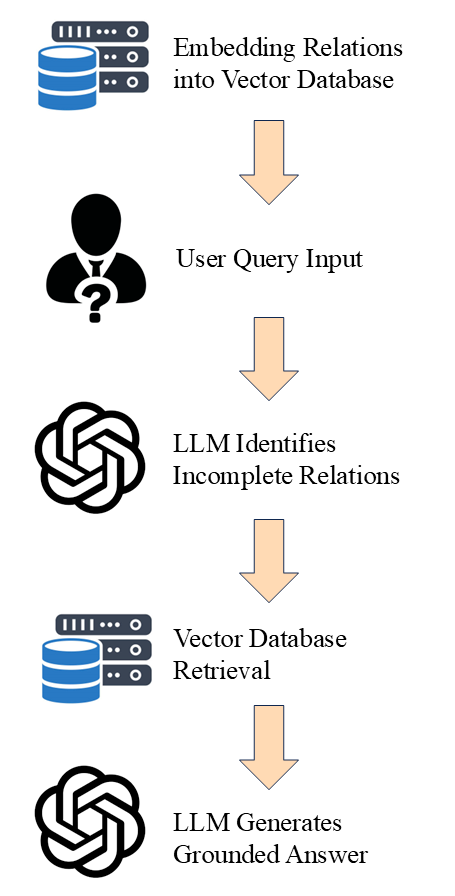
\includegraphics[width=0.7\linewidth]{images/answer_generation.png}
			
		\end{columns}
		
	\end{frame}
	
	\begin{frame}{Experimental Settings}
		
		\scriptsize
		\centering
		
		{\textbf{\textcolor{blue!70}{Table I: Configuration of the Proposed Method}}}
		
		\vspace{0.15cm}
		
		\begin{tabular}{|l|l|}
			\hline
			\textbf{\textcolor{purple!80}{Component}} & \textbf{\textcolor{purple!80}{Configuration}} \\
			\hline
			Graph Database & Neo4j \\
			Vector Database & FAISS \\
			Vector Similarity Metric & Euclidean Distance (L2) \\
			Embeddings & text-embedding-ada-002 \\
			Knowledge Graph Construction & GPT-4o \\
			Relation Extraction & GPT-4o \\
			Answer Generation Model & GPT-3.5-turbo \\
			\hline
		\end{tabular}
		
		\vspace{0.5cm}
		
		{\textbf{\textcolor{blue!70}{Table II: Configuration of the Baseline RAG Approach}}}
		
		\vspace{0.15cm}
		
		\begin{tabular}{|l|l|}
			\hline
			\textbf{\textcolor{purple!80}{Component}} & \textbf{\textcolor{purple!80}{Configuration}} \\
			\hline
			Vector Database & Weaviate \\
			Vector Similarity Metric & Euclidean Distance (L2) \\
			Embeddings & text-embedding-ada-002 \\
			Answer Generation Model & GPT-3.5-turbo \\
			\hline
		\end{tabular}
		
	\end{frame}
	
	\begin{frame}{Evaluation Metrics: RAGAS Framework}
		
		\scriptsize
		
		\begin{itemize}
			
			\item \textbf{\textcolor{blue!70}{RAGAS Framework}}
			\begin{itemize}
				\item \textbf{\textcolor{teal!80}{Answer Similarity}}:
				semantic similarity between generated answer and ground truth,
				computed using cosine similarity of embeddings
				
				\vspace{0.15cm}
				
				\item \textbf{\textcolor{teal!80}{Answer Correctness}}:
				weighted combination of factual correctness and semantic similarity
			\end{itemize}
			
			\vspace{0.25cm}
			
			\textbf{\textcolor{purple!80}{Factual Correctness (F1 Score)}}
			
			\vspace{0.1cm}
			
			\[
			\text{Precision} = \frac{TP}{TP + FP}
			\]
			
			\[
			\text{Recall} = \frac{TP}{TP + FN}
			\]
			
			\[
			F1 = 2 \times \frac{\text{Precision} \times \text{Recall}}
			{\text{Precision} + \text{Recall}}
			\]
			
			\textbf{\textcolor{purple!80}{Answer Correctness Score}}
			
			\vspace{0.1cm}
			
			\[
			\text{Answer Correctness}
			= w_f \times F1
			+ w_s \times \text{Semantic Similarity}
			\]
			
			\[
			w_f = 0.75 \quad,\quad w_s = 0.25
			\]
			
		\end{itemize}
		
	\end{frame}
	
	\begin{frame}{Evaluation Metrics: LLM Evaluator}
		
		\scriptsize
		
		\begin{itemize}
			
			\item \textbf{\textcolor{blue!70}{LLM Evaluator}}:
			head-to-head comparison without predefined ground truth
			
			\vspace{0.2cm}
			
			\item \textbf{\textcolor{teal!80}{Methodology}}:
			\begin{itemize}
				\item LLM receives the question and answers from both methods
				\item LLM selects the superior answer
				\item repeated for all questions in the dataset
			\end{itemize}
			
			\vspace{0.25cm}
			
			\item \textbf{\textcolor{teal!80}{Qualitative Dimensions}}:
			\begin{itemize}
				\item \textbf{\textcolor{purple!80}{Comprehensiveness}}: depth and completeness
				\item \textbf{\textcolor{purple!80}{Empowerment}}: usefulness and actionability
				\item \textbf{\textcolor{purple!80}{Directness}}: clarity and interpretability
				\item \textbf{\textcolor{purple!80}{Diversity}}: variation in responses
			\end{itemize}
			
			\vspace{0.25cm}
			
			\item \textbf{\textcolor{gray!80}{Outcome}}:
			aggregated win/loss counts comparing proposed method and baseline
			
		\end{itemize}
		
	\end{frame}
	
	\begin{frame}{RAGAS Results}
		
		\scriptsize
		\centering
		
		{\textbf{\textcolor{blue!70}{Table III: RAGAS Framework Results on Both Datasets}}}
		
		\vspace{0.15cm}
		
		\begin{tabular}{|l|c|c|c|c|}
			\hline
			\textbf{\textcolor{purple!80}{Metric}} &
			\textbf{\textcolor{teal!80}{Proposed}} &
			\textbf{\textcolor{gray!80}{Baseline}} &
			\textbf{\textcolor{teal!80}{Proposed}} &
			\textbf{\textcolor{gray!80}{Baseline}} \\
			\hline
			& \multicolumn{2}{c|}{\textbf{\textcolor{blue!60}{Our Dataset}}} &
			\multicolumn{2}{c|}{\textbf{\textcolor{blue!60}{MuSiQue Testset}}} \\
			\hline
			Correctness & \textcolor{teal!80}{0.649} & 0.493 & \textcolor{teal!80}{0.477} & 0.382 \\
			Similarity  & \textcolor{teal!80}{0.948} & 0.905 & \textcolor{teal!80}{0.928} & 0.876 \\
			\hline
		\end{tabular}
		
		\vspace{0.45cm}
		
		{\textbf{\textcolor{blue!70}{Table IV: RAGAS Metric Comparison Counts}}}
		
		\vspace{0.15cm}
		
		\begin{tabular}{|l|c|c|c|c|}
			\hline
			\textbf{\textcolor{purple!80}{Metric}} &
			\textbf{\textcolor{teal!80}{Proposed}} &
			\textbf{\textcolor{gray!80}{Baseline}} &
			\textbf{\textcolor{teal!80}{Proposed}} &
			\textbf{\textcolor{gray!80}{Baseline}} \\
			\hline
			& \multicolumn{2}{c|}{\textbf{\textcolor{blue!60}{Our Dataset}}} &
			\multicolumn{2}{c|}{\textbf{\textcolor{blue!60}{MuSiQue Testset}}} \\
			\hline
			Correctness & \textcolor{teal!80}{186} & 110 & \textcolor{teal!80}{17} & 8 \\
			Similarity  & \textcolor{teal!80}{170} & 126 & \textcolor{teal!80}{18} & 7 \\
			\hline
		\end{tabular}
		
	\end{frame}
	
	\begin{frame}{LLM Evaluator Results}
		
		\scriptsize
		\centering
		
		{\textbf{\textcolor{blue!70}{Table V: LLM Evaluator Results on Both Datasets}}}
		
		\vspace{0.2cm}
		
		\begin{tabular}{|l|c|c|c|c|}
			\hline
			\textbf{\textcolor{purple!80}{Dimension}} &
			\textbf{\textcolor{teal!80}{P}} &
			\textbf{\textcolor{gray!80}{B}} &
			\textbf{\textcolor{teal!80}{P}} &
			\textbf{\textcolor{gray!80}{B}} \\
			\hline
			& \multicolumn{2}{c|}{\textbf{\textcolor{blue!60}{Our Dataset}}} &
			\multicolumn{2}{c|}{\textbf{\textcolor{blue!60}{MuSiQue Testset}}} \\
			\hline
			Comprehensiveness & \textcolor{teal!80}{224} & 72 & \textcolor{teal!80}{20} & 5 \\
			Diversity          & 155 & 141 & 14 & 11 \\
			Empowerment        & \textcolor{teal!80}{246} & 50 & \textcolor{teal!80}{21} & 4 \\
			Directness         & \textcolor{teal!80}{162} & 134 & \textcolor{teal!80}{16} & 9 \\
			\hline
		\end{tabular}
		
		\vspace{0.25cm}
		
		{\textbf{\textcolor{gray!80}{\scriptsize
					P: proposed method wins \quad
					B: baseline method wins
		}}}
		
	\end{frame}
	
	\begin{frame}{References}
		\bibliographystyle{apalike}
		\bibliography{References.bib}
	\end{frame}
	
	\begin{frame}{From Local to Global: A GraphRAG Approach to Query-Focused Summarization}
		
		\vspace{0.4em}
		
		\begin{itemize}
			\item \textbf{Authors:} Darren Edge, Ha Trinh, et al. (Microsoft Research)
			
			\item \textbf{Problem:} Conventional RAG performs well for fact‑level queries but struggles with \emph{global questions} that require understanding an entire corpus
			\begin{itemize}
				\item Example: ``What are the main themes in this dataset?''
			\end{itemize}
			
			\item \textbf{Objective:} Design a scalable QA framework over private text corpora that handles
			\begin{itemize}
				\item \textbf{Query generality:} from specific facts to high‑level themes
				\item \textbf{Data scale:} collections with 1M+ tokens
			\end{itemize}
			
			\item \textbf{Core Innovation — GraphRAG:} A graph‑based index built using LLMs
			\begin{itemize}
				\item \textbf{Entity Knowledge Graph:} entities and relations extracted from documents
				\item \textbf{Community Summaries:} pre‑computed summaries of related entity groups
			\end{itemize}
		\end{itemize}
		
	\end{frame}
	
	\begin{frame}{The Gap in Conventional Vector RAG}
		
		\begin{itemize}
			\item \textbf{Mechanism:} Standard vector RAG retrieves documents based on semantic similarity in embedding space.
			
			\item \textbf{The Sensemaking Problem:} Global tasks require understanding interconnected entities, events, and themes across an entire corpus.
			
			\item \textbf{Failure Mode:} Vector RAG is optimized for fact retrieval, not query-focused summarization over large document collections.
		\end{itemize}
		
	\end{frame}
	
	\begin{frame}{The GraphRAG Pipeline Overview}
		
		\begin{columns}[T,onlytextwidth]
			
			\begin{column}{0.50\textwidth}
				\begin{itemize}
					\item \textbf{Indexing Phase:}
					\begin{itemize}
						\item Source Documents $\rightarrow$ Text Chunks
						\item Entity \& Relationship Extraction
						\item Knowledge Graph Construction
						\item Community Detection
						\item Community Summarization
					\end{itemize}
					
					\item \textbf{Query Phase:}
					\begin{itemize}
						\item User Query $\rightarrow$ Community Answers (Map)
						\item Aggregation into Global Answer (Reduce)
					\end{itemize}
					
					\item \textbf{Core Strength:} Leverages graph modularity for parallel, hierarchical summarization.
				\end{itemize}
			\end{column}
			
			\begin{column}{0.45\textwidth}
				\centering
				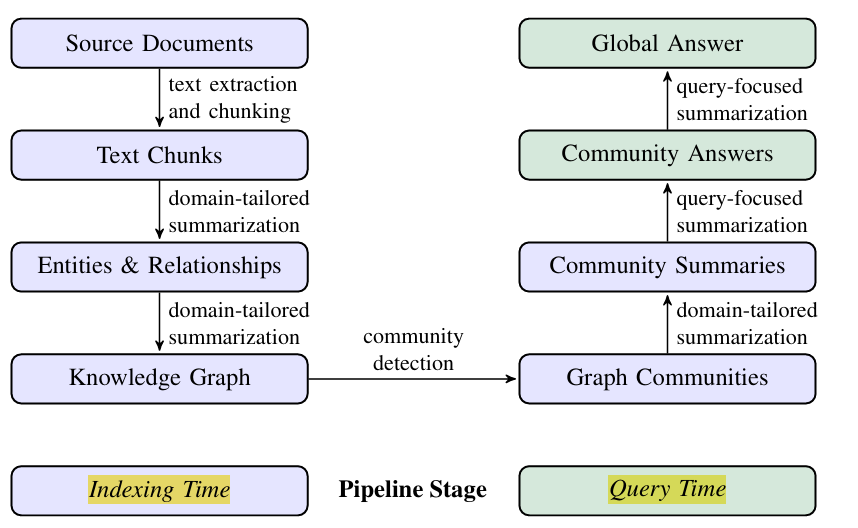
\includegraphics[width=\linewidth]{images/from_local_to_global_fig1.png}
				\vspace{0.3em}
				{\scriptsize Figure 1: High-level GraphRAG indexing and query pipeline.}
				
			\end{column}
			
		\end{columns}
		
	\end{frame}
	
	\begin{frame}{Entity Extraction and the ``Gleaning'' Technique}
		
		\begin{itemize}
			\item \textbf{Chunking Strategy:} Documents are split into 600-token chunks to maximize information recall. (larger chunks reduce cost but may degrade information recall)
			
			\item \textbf{Extraction:} LLM extracts entities (name, type, description) and relationships (description, strength).
			
			\item \textbf{Self-Reflection (Gleaning):} 
			\begin{itemize}
				\item LLM evaluates whether entities were missed.
				\item Additional extraction passes recover missing elements.
			\end{itemize}
		\end{itemize}
		
	\end{frame}
	
	\begin{frame}{From Unstructured Text to a Knowledge Graph}
		
		\begin{itemize}
			\item \textbf{Abstractive Summarization:} Entity and relationship extraction acts as a conceptual summary of the text.
			
			\item \textbf{Aggregation:} Repeated entities and relationships across documents are merged into unified nodes and edges.
			
			\item \textbf{Resilience:} Despite simple string matching, duplicate entities naturally cluster during community detection.
		\end{itemize}
		
	\end{frame}
	
	\begin{frame}{Partitioning the Graph with the Leiden Algorithm}
		
		\begin{columns}[T,onlytextwidth]
			
			\begin{column}{0.50\textwidth}
				\begin{itemize}
					\item \textbf{Modular Partitioning:} Strongly connected nodes are grouped into communities.
					
					\item \textbf{Leiden Algorithm:} Applied recursively to generate a hierarchy of communities.
					
					\item \textbf{Scalability:} Enables divide-and-conquer summarization from root-level (global) to leaf-level (local) communities.
				\end{itemize}
			\end{column}
			
			\begin{column}{0.45\textwidth}
				\centering
				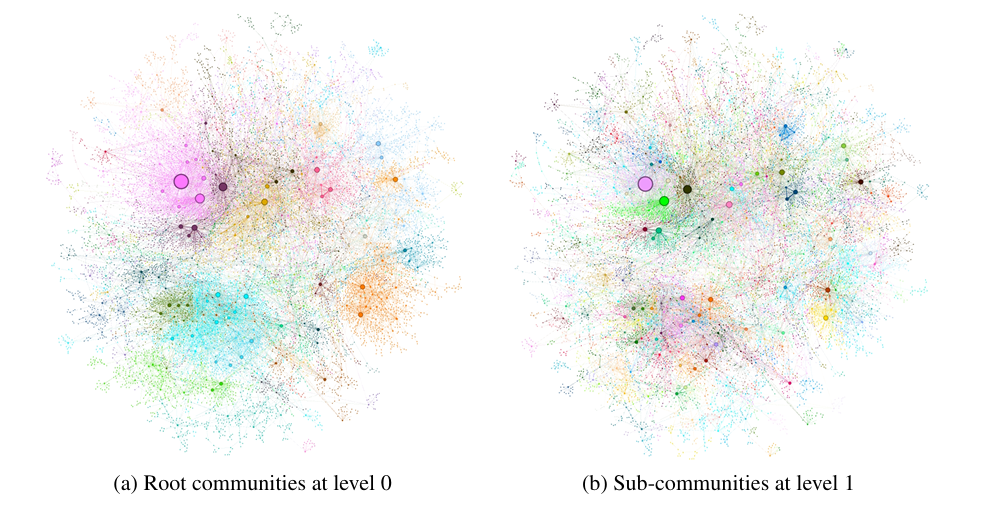
\includegraphics[width=\linewidth]{images/from_local_to_global_fig3.png}
				
				\vspace{0.2em}
				{\scriptsize \textit{Figure 4: Hierarchical community structure induced by the Leiden algorithm}}
			\end{column}
			
		\end{columns}
		
	\end{frame}
	
	\begin{frame}{Generating Hierarchical Community Reports}
		
		\begin{itemize}
			\item \textbf{Report Structure:}
			\begin{itemize}
				\item Executive summary
				\item Impact rating
				\item Detailed findings grounded in graph data
			\end{itemize}
			
			\item \textbf{Bottom-Up Generation:} Leaf-level summaries emphasize entity and relationship details.
			
			\item \textbf{Context Management:} Higher-level summaries replace detailed content with concise sub-community summaries.
		\end{itemize}
		
	\end{frame}
	
	\begin{frame}{Executing Global Queries via Map-Reduce}
		
		\begin{itemize}
			\item \textbf{Preparation:} Community summaries are shuffled and chunked to balance context distribution.
			
			\item \textbf{Map Step:} Parallel generation of intermediate answers with helpfulness scores (0–100).
			
			\item \textbf{Reduce Step:} High-scoring answers are filtered, ranked, and merged to produce the final response.
		\end{itemize}
		
	\end{frame}
	
	\begin{frame}{Benchmarking Global Sensemaking}
		
		\begin{itemize}
			\item \textbf{Motivation:} Existing RAG benchmarks focus on factoid retrieval.
			
			\item \textbf{Adaptive Evaluation:}
			\begin{itemize}
				\item Generate hypothetical personas
				\item Identify persona-specific tasks
				\item Create global, corpus-level questions
			\end{itemize}
			
			\item \textbf{Scale:} 125 questions generated per dataset (Podcasts and News).
		\end{itemize}
		
	\end{frame}
	
	\begin{frame}{Defining Evaluation Criteria}
		
		\begin{itemize}
			\item \textbf{Comprehensiveness:} Coverage of all relevant aspects of the question.
			
			\item \textbf{Diversity:} Variety of insights, viewpoints, and themes.
			
			\item \textbf{Empowerment:} Ability to support informed reasoning with evidence.
			
			\item \textbf{Directness (Control):} Conciseness and specificity used to validate other metrics.
		\end{itemize}
		
	\end{frame}
	
	\begin{frame}{Performance Comparison: GraphRAG vs. Vector RAG}
		
		\begin{columns}[T,onlytextwidth]
			
			\begin{column}{0.50\textwidth}
				\begin{itemize}
					\item \textbf{Dominance:} GraphRAG outperforms vector RAG in
					\begin{itemize}
						\item Comprehensiveness (72--83\% win rate)
						\item Diversity (62--82\% win rate)
					\end{itemize}
					
					\item \textbf{Trade-Off:} Vector RAG excels in Directness but lacks global context.
					
					\item \textbf{Consistency:} Results hold across Podcast and News datasets.
				\end{itemize}
			\end{column}
			
			\begin{column}{0.45\textwidth}
				\centering
				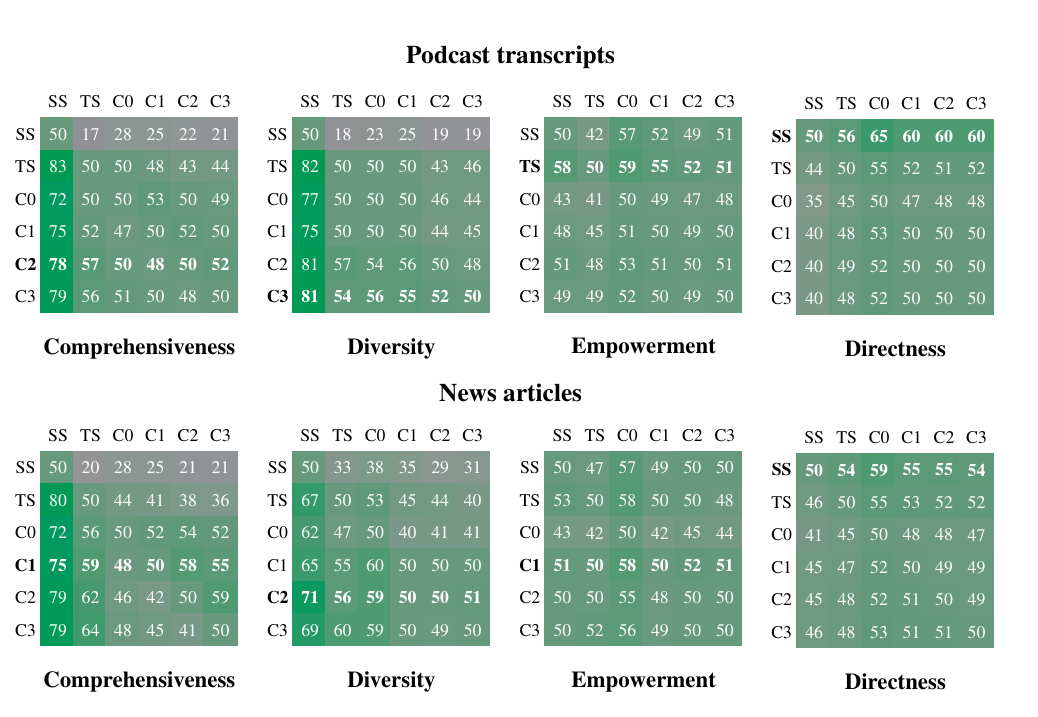
\includegraphics[width=\linewidth]{images/from_local_to_global_fig2.png}
				
				\vspace{0.2em}
				{\scriptsize \textit{Figure 2: Win-rate comparison across evaluation metrics}}
			\end{column}
			
		\end{columns}
		
	\end{frame}
	
	\begin{frame}{Balancing Performance and Token Cost}
		
		\begin{itemize}
			\item \textbf{Root-Level Efficiency (C0):}
			\begin{itemize}
				\item Requires 9x–43x fewer tokens than full text summarization
				\item Still outperforms vector RAG
			\end{itemize}
			
			\item \textbf{Hierarchical Scaling:} Lower-level summaries (C3) use 26–33\% fewer tokens with best performance.
			
			\item \textbf{Conclusion:} C0 summaries provide an efficient entry point for iterative sensemaking.
		\end{itemize}
		
	\end{frame}
	
	\begin{frame}{Validating Results with Claim-Based Measures}
		
		\begin{itemize}
			\item \textbf{Factual Claims:} Verifiable statements extracted using Claimify\textsuperscript{1}.
			
			\item \textbf{Validation Results:}
			\begin{itemize}
				\item Higher number of unique claims (Comprehensiveness)
				\item More claim clusters (Diversity)
			\end{itemize}
			
			\item \textbf{Alignment:} 78\% agreement between claim-based metrics and LLM-as-a-judge scores.
		\end{itemize}
		
		\vfill
		{\tiny
			\textsuperscript{1}\,
			Claimify (Metropolitansky \& Larson, 2025) is an LLM-based method that identifies
			sentences containing at least one factual claim and decomposes them into simple,
			self-contained, verifiable claims.
		}
		
	\end{frame}
	
	\begin{frame}{Key Takeaways}
		
		\begin{itemize}
			\item Vector RAG fails on global sensemaking tasks.
			
			\item GraphRAG introduces a scalable, graph-based summarization framework.
			
			\item Hierarchical community summaries enable efficient, global reasoning over 1M+ tokens.
			
			\item GraphRAG significantly improves comprehensiveness and diversity while controlling token cost.
		\end{itemize}
		
	\end{frame}
	
	\begin{frame}{SoK: Privacy Risks and Mitigations in Retrieval-Augmented Generation Systems}
		
		\begin{itemize}
			\item \textbf{Authors:} Andreea-Elena Bodea, Stephen Meisenbacher, Alexandra Klymenko, Florian Matthes  
			(Technical University of Munich)
			
			\item \textbf{Goal:} First systematization of privacy risks, mitigations, and evaluation strategies in RAG systems via a systematic literature review (72 papers).
			
			\item \textbf{Key Artifacts:}
			\begin{itemize}
				\item Taxonomy of RAG privacy risks
				\item RAG privacy process diagram
			\end{itemize}
		\end{itemize}
		
	\end{frame}
	
	\begin{frame}{The Two-Sided Coin: Leakage vs. Adversarial Manipulation}
		
		\begin{itemize}
			\item \textbf{Threat Landscape:} Privacy risks fall into:
			\begin{itemize}
				\item \textbf{Leakage:} Inherent system vulnerabilities
				\item \textbf{Adversarial Manipulation:} Malicious attacks
			\end{itemize}
			
			\item \textbf{Conceptual Difference:}
			\begin{itemize}
				\item Leakage focuses on \emph{what} is exposed
				\item Attacks focus on \emph{how} exposure is triggered
			\end{itemize}
			
			\item \textbf{Leakage Spectrum:} Sensitive data may leak at any pipeline checkpoint (chunking, encoding, retrieval, generation).
		\end{itemize}
		
	\end{frame}
	
	\begin{frame}{Risk Point 1: Dataset Leakage}
		
		\begin{itemize}
			\item \textbf{Technical Risks:}
			\begin{itemize}
				\item Insecure storage (e.g., unprotected cloud drives)
				\item Weak internal access controls
			\end{itemize}
			
			\item \textbf{PII Exposure:} Non-malicious leakage when sensitive data is indexed without masking or sanitization.
			
			\item \textbf{Mitigations:}
			\begin{itemize}
				\item Automated PII detection and redaction
				\item Strong access control policies
				\item Synthetic data generation
				\item Text rewriting to preserve semantics while removing sensitivity
			\end{itemize}
		\end{itemize}
		
	\end{frame}
	
	\begin{frame}{Risk Point 2: Vector Database Leakage}
		
		\begin{itemize}
			\item \textbf{Embedding Risk:} Model memorization enables reconstruction of proprietary data from embeddings.
			
			\item \textbf{Insecure Search:} Queries similar to confidential content may retrieve sensitive vectors.
			
			\item \textbf{Mitigations:}
			\begin{itemize}
				\item Differential Privacy (DP) during embedding
				\item Synthetic data usage
				\item Role-based access control on vector stores
				\item injection of redundant non-sensitive examples into the vector stores
				\item simple duplication ( to prevent statistical identification of unique outliers)
			\end{itemize}
		\end{itemize}
		
	\end{frame}
	
	\begin{frame}{Risk Point 3: Retrieved Chunk Leakage}
		
		\begin{itemize}
			\item \textbf{Pipeline Risk:} Sensitive chunks retrieved and passed directly to the LLM.
			
			\item \textbf{Adversarial Potential:} Manipulation of retrieval or reranking to surface confidential content.
			
			\item \textbf{Balance Point:} Retrieval is the last stage to control exposure before generation.
			
			\item \textbf{Mitigations:}
			\begin{itemize}
				\item Indexing and reranking modifications
				\item Differential Privacy at cross-attention or reranking stages
			\end{itemize}
		\end{itemize}
		
	\end{frame}
	
	\begin{frame}{Risk Point 4: Answer Leakage}
		
		\begin{itemize}
			\item \textbf{LLM Propagation:} Models may introduce sensitive information not present in retrieved chunks.
			
			\item \textbf{Post-Generation Risk:} Leakage via logs, cached outputs, or conversation histories.
			
			\item \textbf{Mitigations:}
			\begin{itemize}
				\item Local LLM deployment
				\item Post-generation guardrails and filtering
				\item Source attribution and citation enforcement
			\end{itemize}
		\end{itemize}
		
	\end{frame}
	
	\begin{frame}{Risk Point 5: Prompt Leakage}
		
		\begin{itemize}
			\item \textbf{User-Side Risk:} Sensitive information in prompts may persist across logs or sessions.
			
			\item \textbf{Mitigations:}
			\begin{itemize}
				\item Prompt anonymization and filtering
				\item Prompt rewriting and paraphrasing
				\item Multi-Party Computation (MPC)
			\end{itemize}
		\end{itemize}
		
	\end{frame}
	
	\begin{frame}{Categorizing Adversarial Manipulation}
		
		\begin{itemize}
			\item \textbf{Direct Attacks:}
			\begin{itemize}
				\item Jailbreaking
				\item Prompt Injection
				\item Data Poisoning
			\end{itemize}
			
			\item \textbf{Inference \& Extraction Attacks:}
			\begin{itemize}
				\item Membership Inference
				\item Data Extraction from outputs
			\end{itemize}
		\end{itemize}
		
	\end{frame}
	
	\begin{frame}{Dynamic Process View: Setup vs. Inference}
		
		\begin{itemize}
			\item \textbf{Pipeline Dependency:} Mitigations at one stage affect all downstream stages.
			
			\item \textbf{Setup Stage (Indexing):}
			\begin{itemize}
				\item Document collection and embedding
				\item Early anonymization may degrade retrieval quality
			\end{itemize}
			
			\item \textbf{Inference Stage (Runtime):}
			\begin{itemize}
				\item Answer filtering and rewriting
				\item Better utility, but late-stage privatization
			\end{itemize}
		\end{itemize}
		
	\end{frame}
	
	\begin{frame}{Assessing Mitigation Maturity and Relevance}
		
		\begin{itemize}
			\item \textbf{Ideation Gap:} Only 24\% of papers discuss deployment costs (latency, overhead).
			
			\item \textbf{Maturity Trends:}
			\begin{itemize}
				\item Dataset leakage and poisoning: more mature
				\item Prompt injection and extraction: less mature
			\end{itemize}
			
			\item \textbf{High-Relevance Techniques:}
			\begin{itemize}
				\item Text filtering and rewriting
				\item Differential Privacy (high interest, low maturity)
			\end{itemize}
		\end{itemize}
		
	\end{frame}
	
	\begin{frame}{Measuring Privacy: Evaluation Metrics}
		
		\begin{itemize}
			\item \textbf{Retrieval Metrics:}
			\begin{itemize}
				\item Accuracy (top-k hit rate)
				\item Precision, Recall, F1-score
			\end{itemize}
			
			\item \textbf{Generation Metrics:}
			\begin{itemize}
				\item ROUGE, BLEU
				\item Rejection Rate
			\end{itemize}
			
			\item \textbf{Attack Metrics:}
			\begin{itemize}
				\item Attack Success Rate (ASR)
				\item Extraction Rate
			\end{itemize}
		\end{itemize}
		
	\end{frame}
	
	\begin{frame}{Technical Trade-offs and Future Research}
		
		\begin{itemize}
			\item \textbf{Utility vs. Privacy:} Need for mitigation ensembles and combined impact analysis.
			
			\item \textbf{Benchmarks:} Lack of RAG-specific privacy benchmarks; reliance on general QA datasets.
			
			\item \textbf{Architectural Complexity:} Privacy implications of agentic and multi-step RAG systems remain open.
		\end{itemize}
		
	\end{frame}
	
	\begin{frame}{References}
		
		\footnotesize
		
		\begin{thebibliography}{9}
			
			\bibitem{bodea2024}
			Bodea, A.-E., Meisenbacher, S., Klymenko, A., and Matthes, F. (2024).\\
			\textit{SoK: Privacy Risks and Mitigations in Retrieval‑Augmented Generation Systems.}\\
			Technical University of Munich, School of Computation, Information and Technology.
			
			\vspace{0.6em}
			
			\bibitem{edge2025}
			Edge, D., Mody, A., Trinh, H., Truitt, S., Cheng, N., Bradley, J., Metropolitansky, D., Chao, A., Ness, R. O., and Larson, J. (2025).\\
			\textit{From Local to Global: A GraphRAG Approach to Query‑Focused Summarization.}\\
			\texttt{arXiv:2404.16130v2 [cs.CL]}, Microsoft Research.
			
		\end{thebibliography}
		
	\end{frame}
	
	\begin{frame}
		\Huge{\centerline{\textbf{Thank You!}}}
	\end{frame}
	
\end{document}
